\documentclass[border=2pt]{standalone}
\usepackage{tikz}
\usetikzlibrary{decorations.pathreplacing,arrows.meta,calc,backgrounds}

\begin{document}
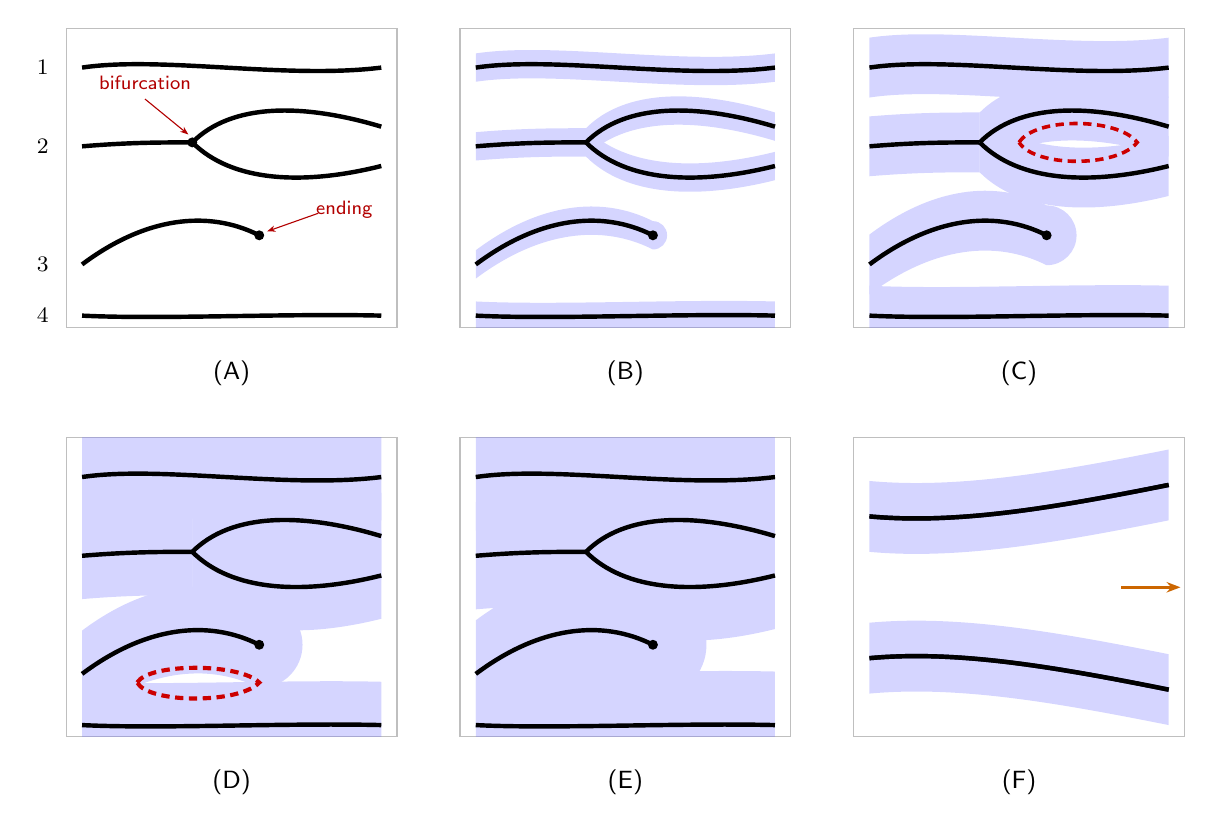
\begin{tikzpicture}[
  ridge/.style={line width=1.6pt, black},
  tube/.style={line width=0pt, fill=blue!25, draw=none},
  cycle mark/.style={densely dashed, line width=1.3pt, red!80!black},
  label style/.style={font=\footnotesize\sffamily},
  panel label/.style={font=\small\sffamily, anchor=north},
  annotation/.style={font=\scriptsize\sffamily, text=red!70!black},
]

% ============================================================
% PANEL LAYOUT: 6 panels in 2 rows x 3 columns
% Row 1: (a) ridge config, (b) t small, (c) t moderate (H1 birth at bifurcation)
% Row 2: (d) t larger (H1 birth at ending region), (e) t large (H1 death), (f) boundary
% ============================================================

\def\pw{4.2}    % panel width
\def\ph{3.8}    % panel height
\def\hgap{0.8}  % horizontal gap
\def\vgap{1.4}  % vertical gap

% Panel origins
\coordinate (P1) at (0,0);
\coordinate (P2) at (\pw+\hgap,0);
\coordinate (P3) at (2*\pw+2*\hgap,0);
\coordinate (P4) at (0,-\ph-\vgap);
\coordinate (P5) at (\pw+\hgap,-\ph-\vgap);
\coordinate (P6) at (2*\pw+2*\hgap,-\ph-\vgap);

% ============================================================
% RIDGE GEOMETRY
% Four ridges: A (top), B (middle, bifurcates into B1 up and B2 down),
% C (lower, ends mid-image), D (bottom, continuous)
% Bifurcation of B creates a small enclosed valley between B1 and B2.
% Ending of C leaves a wide gap between C-end and D, delaying H1.
% ============================================================

% Macro: draw ridges at shift (#1,#2)
\newcommand{\drawridges}[2]{%
  \begin{scope}[shift={(#1,#2)}]
    % Ridge A
    \draw[ridge] (0.2,3.3) .. controls (1.2,3.45) and (2.8,3.15) .. (4.0,3.3);
    % Ridge B stem
    \draw[ridge] (0.2,2.3) .. controls (0.8,2.35) and (1.2,2.35) .. (1.6,2.35);
    % Ridge B1 (upper branch) — diverges then converges to form enclosed pocket
    \draw[ridge] (1.6,2.35) .. controls (2.1,2.85) and (3.0,2.85) .. (4.0,2.55);
    % Ridge B2 (lower branch) — mirrors B1, converging on right
    \draw[ridge] (1.6,2.35) .. controls (2.1,1.85) and (3.0,1.80) .. (4.0,2.05);
    % Ridge C — arches away from D, ends at x~2.45
    % Close to D at left (gap=0.65), far in middle (gap~1.28), endpoint gap=1.00
    \draw[ridge] (0.2,0.80) .. controls (1.0,1.40) and (1.8,1.50) .. (2.45,1.17);
    \fill[black] (2.45,1.17) circle (1.8pt);
    % Ridge D
    \draw[ridge] (0.2,0.15) .. controls (1.2,0.10) and (2.8,0.18) .. (4.0,0.15);
  \end{scope}%
}

% Macro: draw tubes of half-width #3 at shift (#1,#2)
% NOTE: caller must set up clipping before invoking this macro
\newcommand{\drawtubes}[3]{%
  \begin{scope}[shift={(#1,#2)}]
  \begin{scope}[transparency group, opacity=0.30]
    % Tube A
    \fill[blue!55]
      (0.2,{3.3+#3}) .. controls (1.2,{3.45+#3}) and (2.8,{3.15+#3}) .. (4.0,{3.3+#3})
      -- (4.0,{3.3-#3}) .. controls (2.8,{3.15-#3}) and (1.2,{3.45-#3}) .. (0.2,{3.3-#3})
      -- cycle;
    % Tube B stem
    \fill[blue!55]
      (0.2,{2.3+#3}) .. controls (0.8,{2.35+#3}) and (1.2,{2.35+#3}) .. (1.6,{2.35+#3})
      -- (1.6,{2.35-#3}) .. controls (1.2,{2.35-#3}) and (0.8,{2.35-#3}) .. (0.2,{2.3-#3})
      -- cycle;
    % Tube B1
    \fill[blue!55]
      (1.6,{2.35+#3}) .. controls (2.1,{2.85+#3}) and (3.0,{2.85+#3}) .. (4.0,{2.55+#3})
      -- (4.0,{2.55-#3}) .. controls (3.0,{2.85-#3}) and (2.1,{2.85-#3}) .. (1.6,{2.35-#3})
      -- cycle;
    % Tube B2
    \fill[blue!55]
      (1.6,{2.35+#3}) .. controls (2.1,{1.85+#3}) and (3.0,{1.80+#3}) .. (4.0,{2.05+#3})
      -- (4.0,{2.05-#3}) .. controls (3.0,{1.80-#3}) and (2.1,{1.85-#3}) .. (1.6,{2.35-#3})
      -- cycle;
    % Tube C (with rounded end — cap centered on ridge endpoint)
    \fill[blue!55]
      (0.2,{0.80+#3}) .. controls (1.0,{1.40+#3}) and (1.8,{1.50+#3}) .. (2.45,{1.17+#3})
      arc(90:-90:#3)
      .. controls (1.8,{1.50-#3}) and (1.0,{1.40-#3}) .. (0.2,{0.80-#3})
      -- cycle;
    % Tube D
    \fill[blue!55]
      (0.2,{0.15+#3}) .. controls (1.2,{0.10+#3}) and (2.8,{0.18+#3}) .. (4.0,{0.15+#3})
      -- (4.0,{0.15-#3}) .. controls (2.8,{0.18-#3}) and (1.2,{0.10-#3}) .. (0.2,{0.15-#3})
      -- cycle;
  \end{scope}
  \end{scope}%
}

% ============================================================
% PANEL (a): Ridge configuration
% ============================================================
\begin{scope}
  \draw[gray!50, thin] (P1) rectangle +(\pw,\ph);
  \drawridges{0}{0}

  % Ridge labels
  \node[label style, anchor=east] at (-0.1,3.3) {$1$};
  \node[label style, anchor=east] at (-0.1,2.3) {$2$};
  \node[label style, anchor=east] at (-0.1,0.80) {$3$};
  \node[label style, anchor=east] at (-0.1,0.15) {$4$};

  % Bifurcation dot and annotation
  \fill[black] (1.6,2.35) circle (1.8pt);
  \draw[-{Stealth[length=3pt]}, red!70!black, thin] (1.0,2.9) -- (1.55,2.45);
  \node[annotation, anchor=south] at (1.0,2.9) {bifurcation};

  % Ridge ending annotation
  \draw[-{Stealth[length=3pt]}, red!70!black, thin] (3.2,1.45) -- (2.55,1.22);
  \node[annotation, anchor=west] at (3.05,1.5) {ending};

  \node[panel label] at ($(P1)+(0.5*\pw,-0.3)$) {(A)};
\end{scope}

% ============================================================
% PANEL (b): Small t --- thin tubes, gaps everywhere
% CLIPPED to panel bounds
% ============================================================
\begin{scope}
  \draw[gray!50, thin] (P2) rectangle +(\pw,\ph);
  % Clip tubes to panel
  \begin{scope}
    \clip (P2) rectangle +(\pw,\ph);
    \drawtubes{\pw+\hgap}{0}{0.18}
  \end{scope}
  \drawridges{\pw+\hgap}{0}

  \node[panel label] at ($(P2)+(0.5*\pw,-0.3)$) {(B)};
\end{scope}

% ============================================================
% PANEL (c): Moderate t --- bifurcation pocket closes, H1 birth (low b)
% CLIPPED to panel bounds
% ============================================================
\begin{scope}
  \draw[gray!50, thin] (P3) rectangle +(\pw,\ph);
  % Clip tubes to panel
  \begin{scope}
    \clip (P3) rectangle +(\pw,\ph);
    \drawtubes{2*\pw+2*\hgap}{0}{0.38}
  \end{scope}
  \drawridges{2*\pw+2*\hgap}{0}

  \begin{scope}[shift={(2*\pw+2*\hgap,0)}]
    % H1 cycle in bifurcation pocket — enlarged to clear white island edges
    \draw[cycle mark]
      (2.10,2.35) .. controls (2.30,2.67) and (3.35,2.67) .. (3.60,2.35)
      .. controls (3.35,2.03) and (2.30,2.03) .. (2.10,2.35);
  \end{scope}

  \node[panel label] at ($(P3)+(0.5*\pw,-0.3)$) {(C)};
\end{scope}

% ============================================================
% PANEL (d): Larger t --- ending gap closes, H1 birth (high b)
% CLIPPED to panel bounds
% ============================================================
\begin{scope}
  \draw[gray!50, thin] (P4) rectangle +(\pw,\ph);
  % Clip tubes to panel
  \begin{scope}
    \clip (P4) rectangle +(\pw,\ph);
    \drawtubes{0}{-\ph-\vgap}{0.55}
  \end{scope}
  \drawridges{0}{-\ph-\vgap}

  \begin{scope}[shift={(0,-\ph-\vgap)}]
    % H1 cycle in ending region (between C and D)
    % At r=0.55: white pocket spans x~0.9–2.2. Cycle through blue encircling white.
    \draw[cycle mark, line width=1.5pt]
      (0.90,0.69) .. controls (1.05,0.94) and (2.20,0.94) .. (2.45,0.69)
      .. controls (2.20,0.42) and (1.05,0.42) .. (0.90,0.69);
  \end{scope}

  \node[panel label] at ($(P4)+(0.5*\pw,-0.3)$) {(D)};
\end{scope}

% ============================================================
% PANEL (e): Large t --- loops die as valleys fill in
% CLIPPED to panel bounds
% ============================================================
\begin{scope}
  \draw[gray!50, thin] (P5) rectangle +(\pw,\ph);
  % Clip tubes to panel
  \begin{scope}
    \clip (P5) rectangle +(\pw,\ph);
    \drawtubes{\pw+\hgap}{-\ph-\vgap}{0.68}
  \end{scope}
  \drawridges{\pw+\hgap}{-\ph-\vgap}

  % (no annotations — deaths explained in caption)

  \node[panel label] at ($(P5)+(0.5*\pw,-0.3)$) {(E)};
\end{scope}

% ============================================================
% PANEL (f): Boundary --- valley open to edge, no H1 forms
% CLIPPED to panel bounds
% ============================================================
\begin{scope}
  \draw[gray!50, thin] (P6) rectangle +(\pw,\ph);

  \begin{scope}[shift={(2*\pw+2*\hgap,-\ph-\vgap)}]
    % Two ridges diverging toward the right edge, leaving valley open
    \draw[ridge] (0.2,2.8) .. controls (1.3,2.7) and (2.5,2.9) .. (4.0,3.2);
    \draw[ridge] (0.2,1.0) .. controls (1.3,1.1) and (2.5,0.9) .. (4.0,0.6);

    % Tubes — clipped to panel
    \begin{scope}
      \clip (0,0) rectangle (\pw,\ph);
      \begin{scope}[transparency group, opacity=0.30]
        \fill[blue!55]
          (0.2,{2.8+0.45}) .. controls (1.3,{2.7+0.45}) and (2.5,{2.9+0.45}) .. (4.0,{3.2+0.45})
          -- (4.0,{3.2-0.45}) .. controls (2.5,{2.9-0.45}) and (1.3,{2.7-0.45}) .. (0.2,{2.8-0.45})
          -- cycle;
        \fill[blue!55]
          (0.2,{1.0+0.45}) .. controls (1.3,{1.1+0.45}) and (2.5,{0.9+0.45}) .. (4.0,{0.6+0.45})
          -- (4.0,{0.6-0.45}) .. controls (2.5,{0.9-0.45}) and (1.3,{1.1-0.45}) .. (0.2,{1.0-0.45})
          -- cycle;
      \end{scope}
    \end{scope}

    % Redraw ridges on top of tubes
    \draw[ridge] (0.2,2.8) .. controls (1.3,2.7) and (2.5,2.9) .. (4.0,3.2);
    \draw[ridge] (0.2,1.0) .. controls (1.3,1.1) and (2.5,0.9) .. (4.0,0.6);

    % Arrow pointing to open boundary — visual cue that valley is not enclosed
    \draw[-{Stealth[length=5pt]}, orange!80!black, line width=1pt] (3.4,1.9) -- (4.15,1.9);
  \end{scope}

  \node[panel label] at ($(P6)+(0.5*\pw,-0.3)$) {(F)};
\end{scope}

\end{tikzpicture}
\end{document}
